% main.tex
% % Configuración para normas APA 7
\usepackage[spanish]{babel}
\usepackage[utf8]{inputenc}
\usepackage[T1]{fontenc}
\usepackage{csquotes}
\usepackage[style=apa, backend=biber]{biblatex}
\addbibresource{../bibliografia.bib}

% Márgenes y formato
\usepackage[a4paper, margin=2.5cm]{geometry}
\usepackage{setspace}
\onehalfspacing

% Encabezado y pie de página
\usepackage{fancyhdr}
\pagestyle{fancy}
\fancyhf{}
\fancyhead[R]{\thepage}

% Fuente recomendada por APA
\usepackage{times}

\documentclass[12pt,man]{apa7}
\usepackage[spanish]{babel}
\usepackage[utf8]{inputenc}
\usepackage{amsmath,amssymb,amsfonts}
\usepackage{graphicx}
\graphicspath{{./EDOs_v6}}
\usepackage{setspace}
\usepackage{fancyhdr}
\usepackage{float}
\usepackage{tikz}
\usepackage{mathtools}
\usepackage{hyperref}

% APA 7th page geometry ya incluida en apa7
\pagestyle{fancy}
\fancyhf{}
\rhead{\thepage}
\renewcommand{\headrulewidth}{0pt}
\doublespacing
\setlength{\parindent}{0.5in}

% 
\begin{document}

% portada.tex
\title{Ecuaciones Diferenciales Homogéneas y Coeficientes Lineales:\\Aplicaciones en Ingeniería de Sistemas}
\shorttitle{Ecuaciones Diferenciales Homogéneas} % Título corto para cabeceras

% Formato correcto para múltiples autores
\authorsnames{Autor 1, Autor 2}
\authorsaffiliations{
{Programa de Ingeniería de Sistemas, Facultad de Ingeniería, Universidad de la Sabana},
{Programa de Ingeniería de Sistemas, Facultad de Ingeniería, Universidad de la Sabana}
}

\course{Curso: XXXXX}
\professor{Profesor: Nombre del Profesor}
\duedate{\today}

% Abstract debe estar antes de maketitle
\abstract{
Las ecuaciones diferenciales homogéneas con coeficientes lineales constituyen una herramienta fundamental en el modelado matemático de sistemas dinámicos. Este documento presenta una revisión teórica y aplicada de estos conceptos, enfatizando su relevancia en el ámbito de la Ingeniería de Sistemas. Se abordan métodos de solución analíticos y se ilustran aplicaciones prácticas en control automático, redes de comunicación y simulación de procesos. Los ejemplos resueltos demuestran la utilidad de estas ecuaciones para describir comportamientos temporales en sistemas complejos.
}

\maketitle


\newpage
% introduccion.tex
\section{Introducción}

Las ecuaciones diferenciales homogéneas con coeficientes lineales representan una clase fundamental de ecuaciones que modelan fenómenos dinámicos en múltiples disciplinas de la ingeniería. En el contexto de la Ingeniería de Sistemas, estas ecuaciones son particularmente relevantes para describir y analizar el comportamiento temporal de sistemas complejos, desde redes de computadoras hasta procesos de manufactura automatizada.

La importancia de estas ecuaciones radica en su capacidad para capturar relaciones causa-efecto en sistemas donde las tasas de cambio dependen linealmente del estado actual. Por ejemplo, en sistemas de control automático, las ecuaciones diferenciales homogéneas permiten modelar la respuesta temporal de controladores PID, la dinámica de sistemas mecánicos amortiguados o la propagación de señales en redes de comunicación.

En el ámbito de la simulación de procesos, estas ecuaciones permiten predecir el comportamiento de sistemas bajo diferentes condiciones iniciales, facilitando la optimización de parámetros y la identificación de posibles fallos antes de la implementación física. La capacidad de resolver analíticamente estas ecuaciones proporciona una ventaja significativa en términos de comprensión del sistema y predicción de su comportamiento a largo plazo.

Este documento presenta una revisión sistemática de los conceptos teóricos fundamentales relacionados con ecuaciones diferenciales homogéneas con coeficientes lineales, sus métodos de solución y aplicaciones prácticas específicas en Ingeniería de Sistemas. El enfoque se centra en proporcionar herramientas matemáticas que permitan a los ingenieros modelar, analizar y predecir el comportamiento de sistemas dinámicos complejos.
% desarrollo.tex
\newpage
\section{Desarrollo}

\subsection{Conceptos Fundamentales}

Una ecuación diferencial homogénea con coeficientes lineales es una ecuación de la forma

\begin{equation}
    a_n \frac{d^n y}{dx^n} + a_{n-1} \frac{d^{n-1} y}{dx^{n-1}} + \cdots + a_1 \frac{dy}{dx} + a_0 y = 0
\end{equation}

donde $a_0, a_1, \ldots, a_n$ son coeficientes constantes y $y$ es una función de $x$.


\subsection{Ecuaciones de Segundo Orden}

Para el caso particular de ecuaciones de segundo orden, la forma general es:

\begin{equation}
    a \frac{d^2 y}{dx^2} + b \frac{dy}{dx} + c y = 0
\end{equation}

La solución se obtiene mediante la ecuación característica:

\begin{equation}
    ar^2 + br + c = 0
\end{equation}

Las raíces de esta ecuación determinan la forma de la solución general:

\begin{itemize}

\item \textbf{Raíces reales distintas} ($b^2 - 4ac > 0$)
\begin{equation}
    y(x) = C_1 e^{r_1 x} + C_2 e^{r_2 x}
\end{equation}

\item \textbf{Raíces reales repetidas} ($b^2 - 4ac = 0$)
\begin{equation}
    y(x) = (C_1 + C_2 x) e^{rx}
\end{equation}

\item \textbf{Raíces complejas conjugadas} ($b^2 - 4ac < 0$)
\begin{equation}
    y(x) = e^{\alpha x} (C_1 \cos(\beta x) + C_2 \sin(\beta x))
\end{equation}

\end{itemize}

\subsection{Aplicación en Sistemas de Control}

En sistemas de control automático, las ecuaciones diferenciales homogéneas modelan la respuesta natural de sistemas de segundo orden. Consideremos un sistema masa-resorte-amortiguador:

\begin{equation}
    m \frac{d^2 x}{dt^2} + c \frac{dx}{dt} + kx = 0
\end{equation}

donde $m$ es la masa, $c$ es el coeficiente de amortiguamiento, y $k$ es la constante del resorte.

La solución de esta ecuación describe el comportamiento transitorio del sistema, crucial para determinar estabilidad y tiempo de respuesta en sistemas de control.

\subsection{Análisis de Redes de Comunicación}

En el modelado de redes de comunicación, las ecuaciones diferenciales homogéneas describen la dinámica de colas y la propagación de señales. Para un sistema de cola M/M/1, la ecuación de estado puede formularse como:

\begin{equation}
    \frac{dP_n(t)}{dt} = \lambda P_{n-1}(t) - (\lambda + \mu) P_n(t) + \mu P_{n+1}(t)
\end{equation}

En estado estacionario, esta ecuación se simplifica a un sistema homogéneo que permite analizar la estabilidad de la red.

% ejersicios.tex
\section{Ejercicios}

\subsection{Ejercicio 1: Sistema Masa-Resorte-Amortiguador}

Resolver
\[
2\frac{d^2x}{dt^2}+8\frac{dx}{dt}+32x=0,\qquad x(0)=0{,}1\;\text{m},\quad x'(0)=0\;\text{m/s}.
\]
\textbf{Solución:} Ecuación característica $r^2+4r+16=0$ con raíces $r=-2\pm2\sqrt{3}\,i$.  
Aplicando condiciones iniciales:
\[
x(t)=e^{-2t}\left(0{,}1\cos(2\sqrt{3}\,t)+\frac{0{,}1}{\sqrt{3}}\sin(2\sqrt{3}\,t)\right).
\]
\begin{figure}[H]
\centering
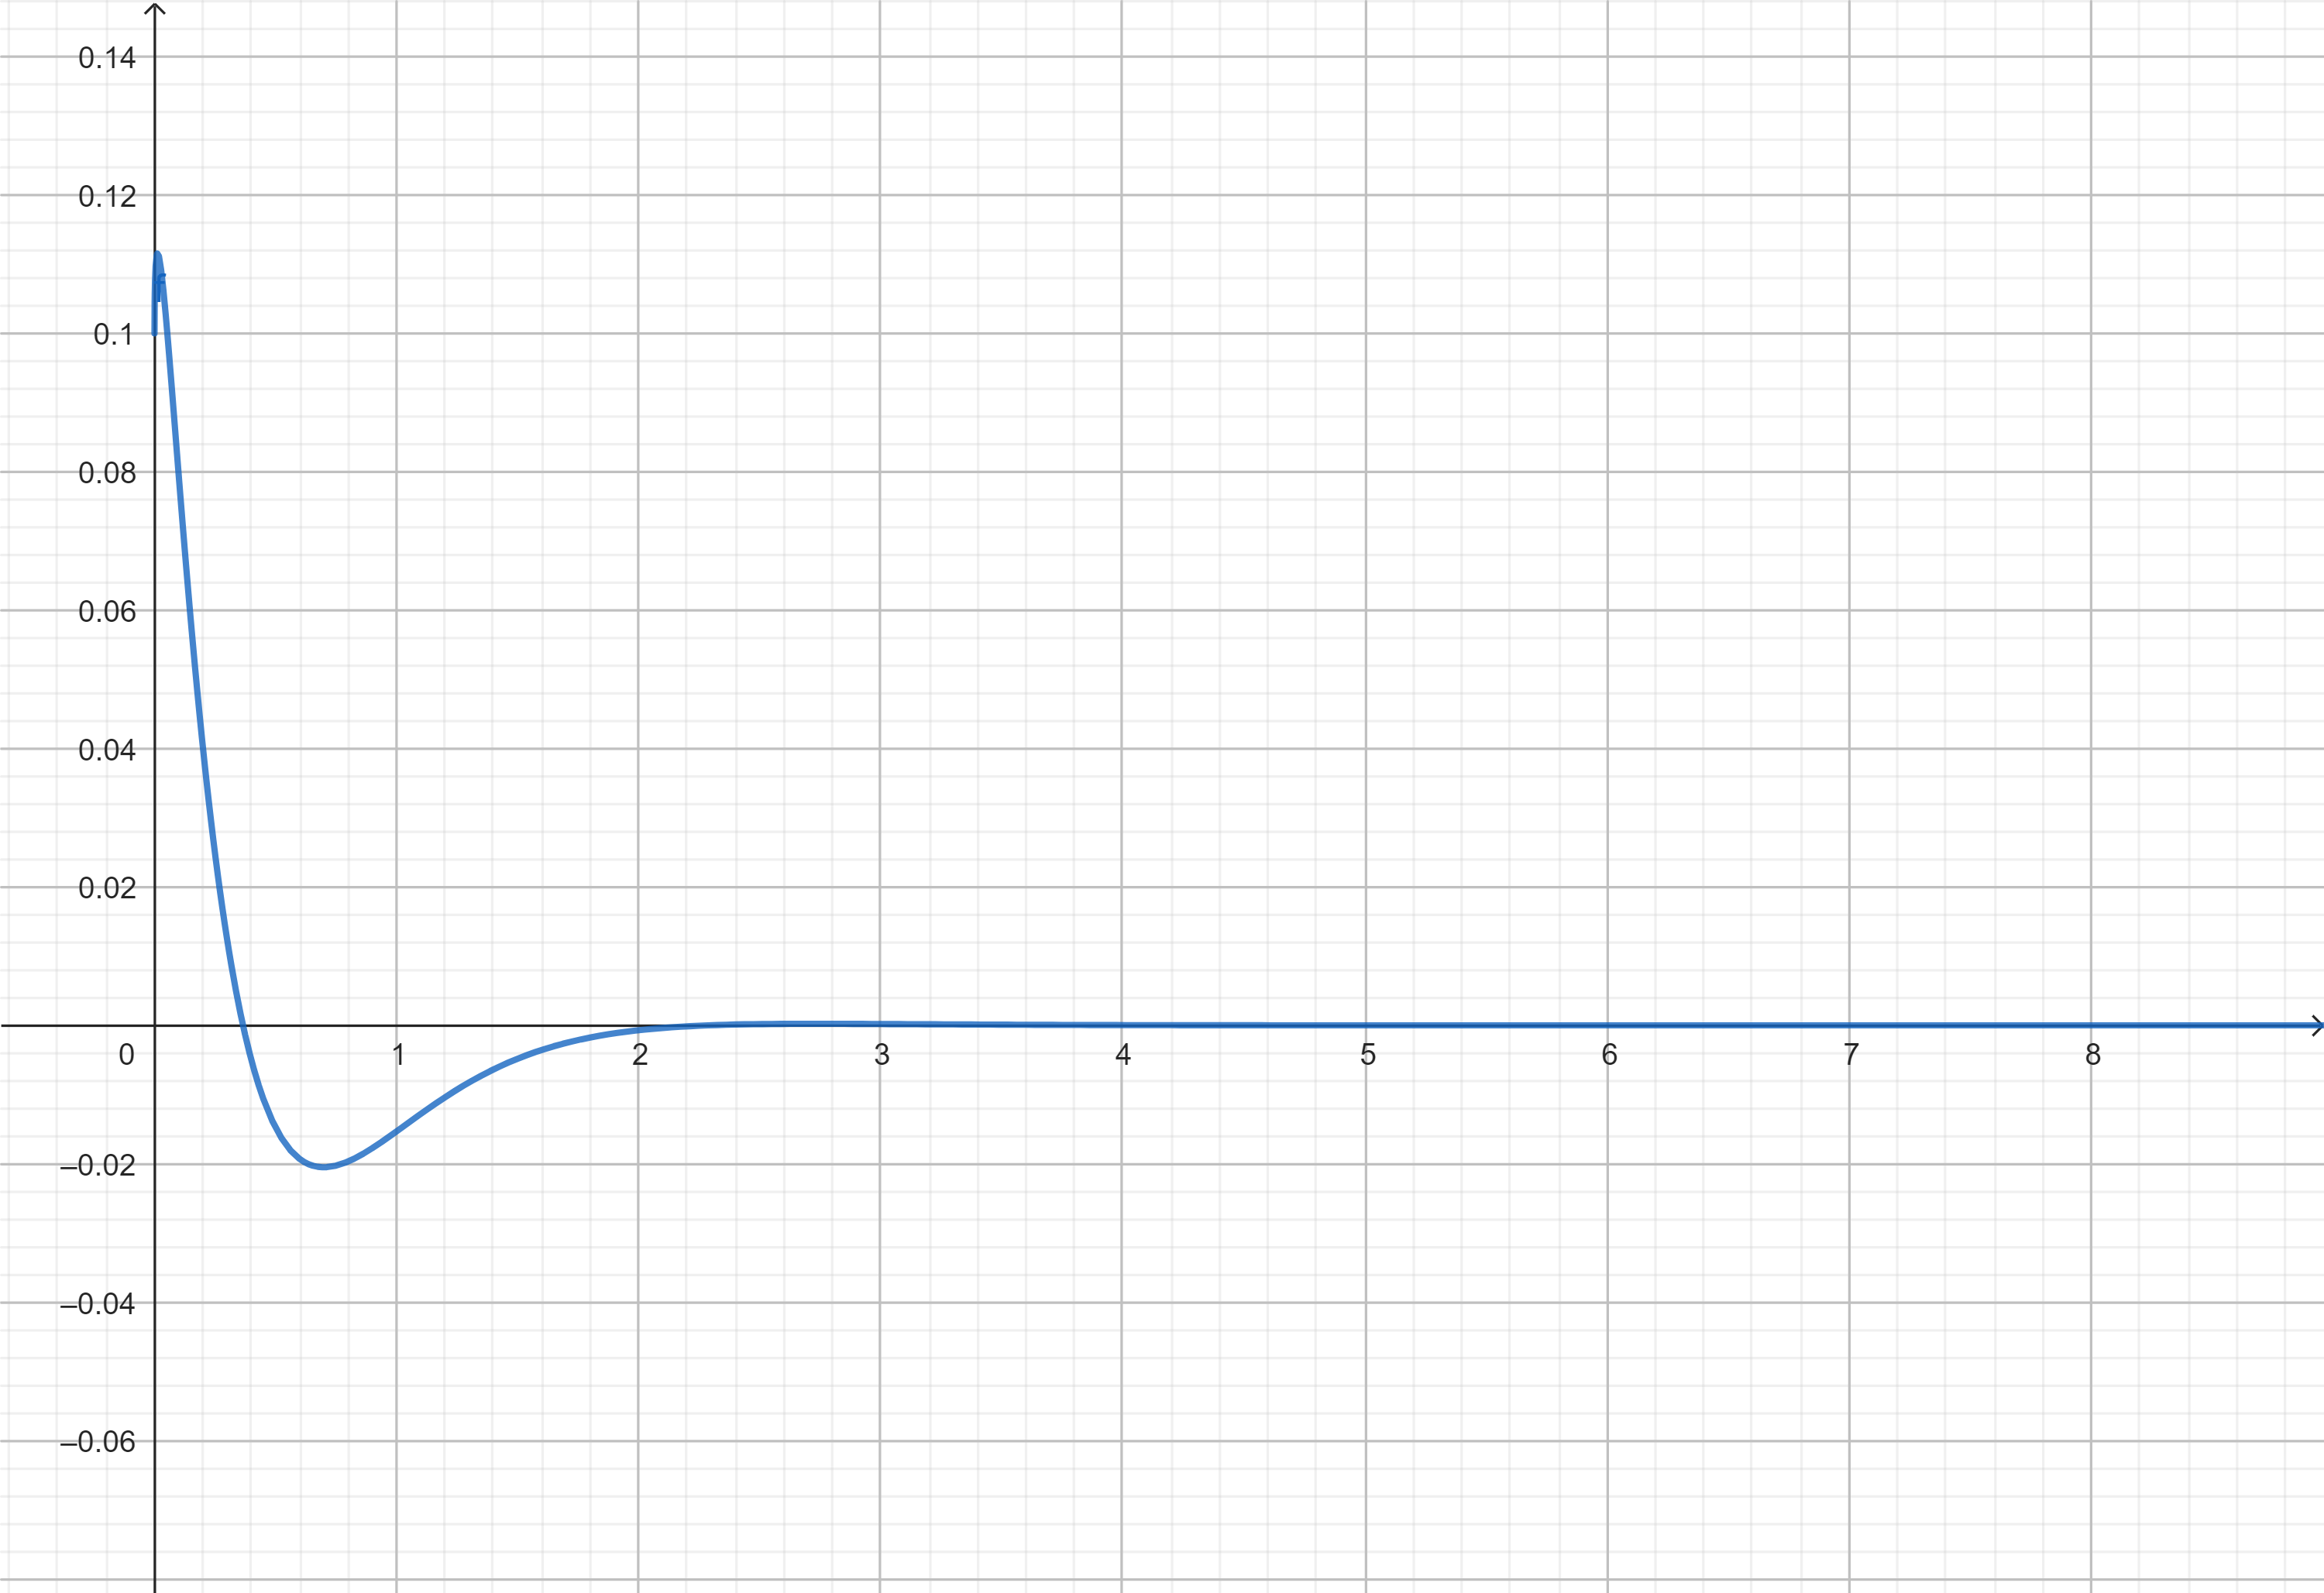
\includegraphics[width=0.8\linewidth]{imagen-ejercicio1.png}
\caption{Respuesta temporal (GeoGebra).}
\end{figure}

\subsection{Ejercicio 2: Circuito RLC en Serie}
Con $R=100\;\Omega$, $L=0{,}5$ H, $C=10\;\mu$F y condiciones iniciales $i(0)=0{,}1$ A, $i'(0)=0$, se obtiene
\[
i(t)=e^{-100t}\bigl(0{,}1\cos(400t)+0{,}025\sin(400t)\bigr).
\]
\begin{figure}[H]
\centering
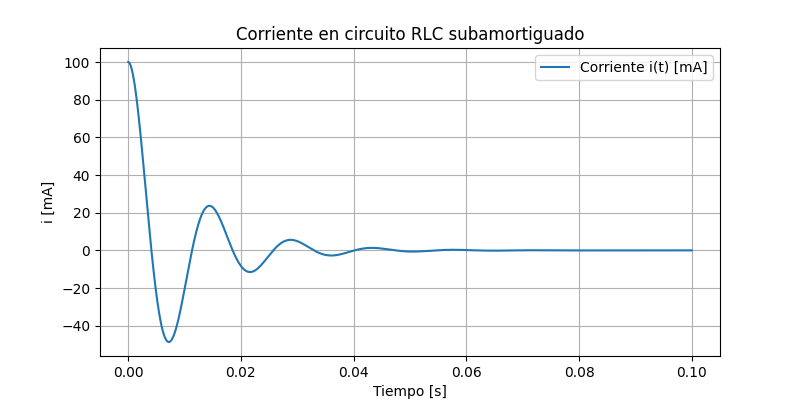
\includegraphics[width=0.8\linewidth]{imagen-ejercicio2.png}
\caption{Corriente en el circuito RLC (Python).}
\end{figure}

\subsection{Ejercicio 3: Control de Nivel}
Para $\frac{dh}{dt}+\frac{k}{A}h=0$ con $A=5$ m$^2$, $k=0{,}5$ m$^2$/s y $h(0)=2$ m:
\[
h(t)=2e^{-0{,}1t}.
\]
\begin{figure}[H]
\centering
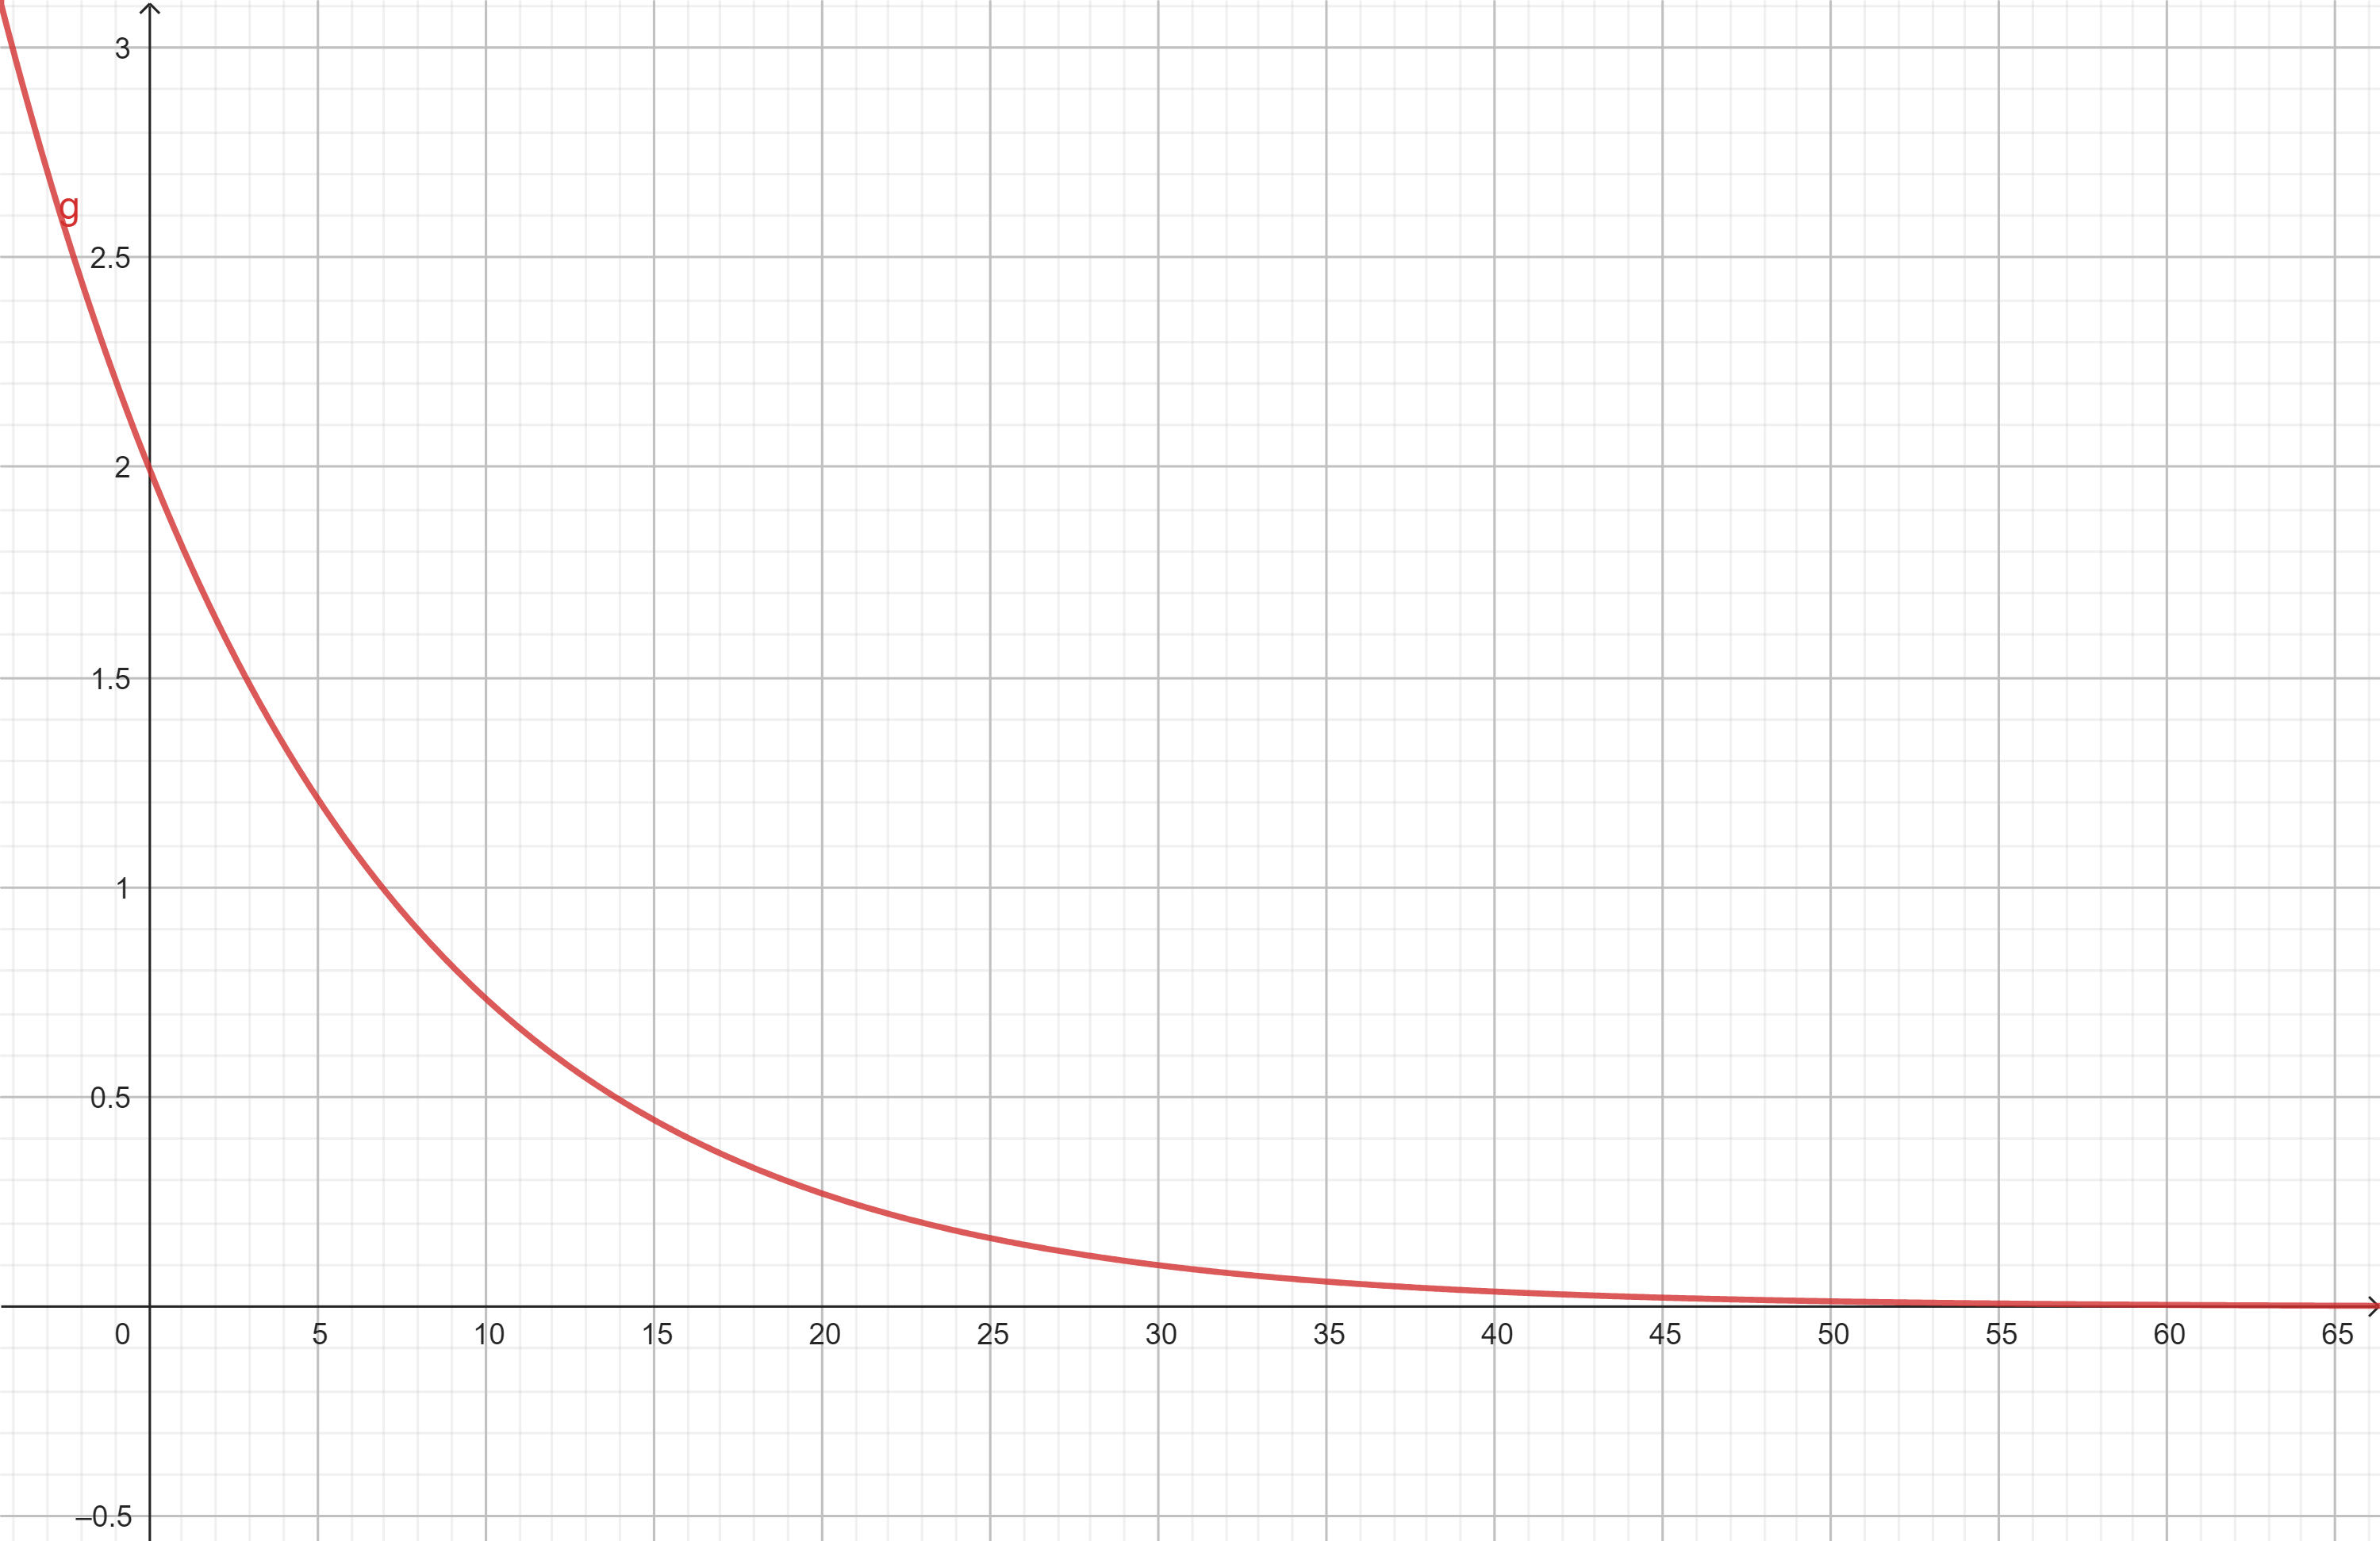
\includegraphics[width=0.8\linewidth]{imagen-ejercicio3.png}
\caption{Nivel del tanque vs.\ tiempo (GeoGebra).}
\end{figure}

\subsection{Ejercicio 4: Decaimiento de Población}
Con $\frac{dP}{dt}=-0{,}05P$ y $P(0)=100\,000$ la población se reduce a la mitad en
\[
t=\frac{\ln 0{,}5}{-0{,}05}\approx13{,}86\;\text{años}.
\]
\begin{figure}[H]
\centering
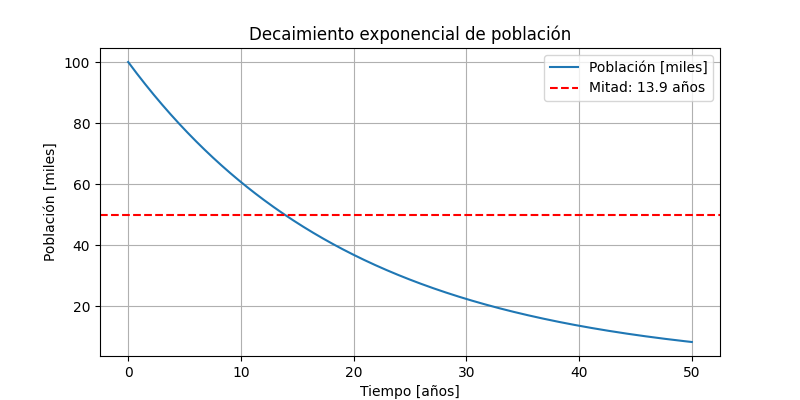
\includegraphics[width=0.8\linewidth]{imagen-ejercicio4.png}
\caption{Decaimiento exponencial (Python).}
\end{figure}

\subsection{Ejercicio 5: Sistema Sobreamortiguado}
Resolviendo
\[
\frac{d^2y}{dt^2}+6\frac{dy}{dt}+8y=0,\qquad y(0)=1,\quad y'(0)=0,
\]
se tiene $r^2+6r+8=0\Rightarrow r_1=-2,\;r_2=-4$, de donde
\[
y(t)=2e^{-2t}-e^{-4t}.
\]
\begin{figure}[H]
\centering
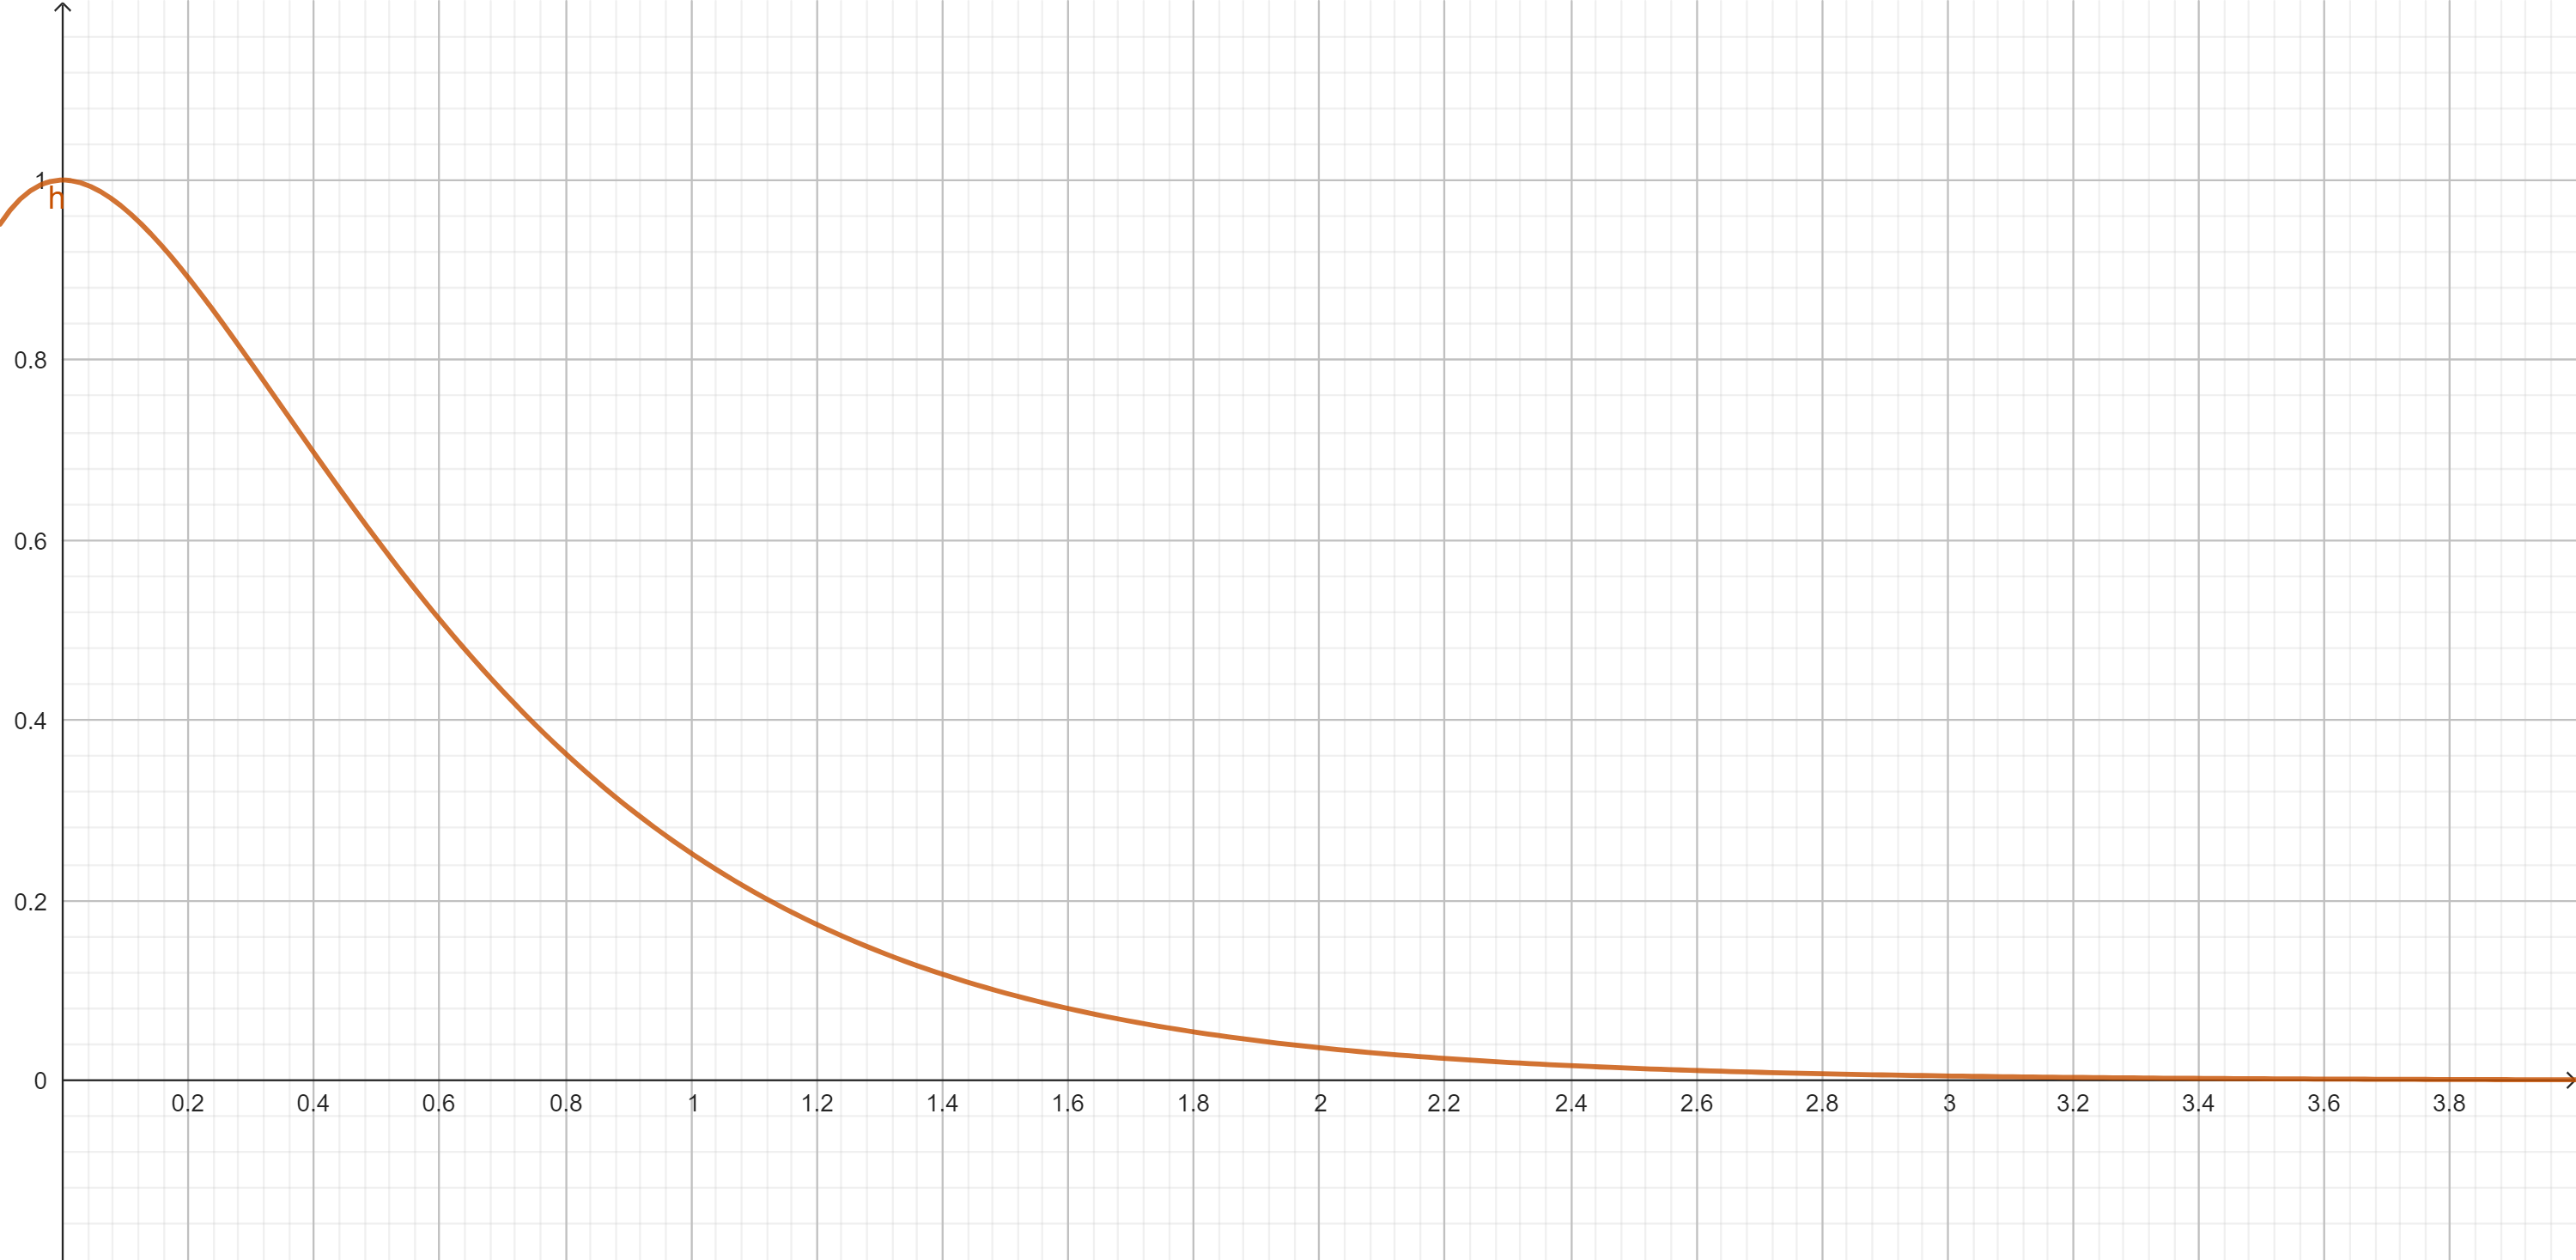
\includegraphics[width=0.8\linewidth]{imagen-ejercicio5.png}
\caption{Respuesta sobreamortiguada (GeoGebra).}
\end{figure}
% conclucion.tex
\section{Conclusión}

Las ecuaciones diferenciales homogéneas con coeficientes lineales constituyen una herramienta matemática fundamental para el análisis y diseño de sistemas en Ingeniería de Sistemas. A través de este documento se ha mostrado cómo modelar comportamientos dinámicos en contextos tan diversos como sistemas mecánicos, circuitos eléctricos, procesos de control y redes de comunicación.

La posibilidad de obtener soluciones analíticas permite comprender, sin ambigüedades, la estabilidad, la respuesta transitoria y el régimen permanente de los sistemas. Los ejemplos prácticos resaltan la utilidad de estos conceptos en la resolución de problemas reales de ingeniería.

Trabajos futuros pueden abordar sistemas no homogéneos, coeficientes variables y el uso de transformadas de Laplace, así como la integración de herramientas computacionales para sistemas de mayor dimensión y complejidad.
% referencias.tex
\newpage
\section{Referencias}

\begin{thebibliography}{}

\bibitem{boyce}
Boyce, W. E., \& DiPrima, R. C. (2021). \textit{Elementary differential equations and boundary value problems} (12th ed.). John Wiley \& Sons.

\bibitem{zill}
Zill, D. G. (2020). \textit{Ecuaciones diferenciales con aplicaciones de modelado} (11ª ed.). Cengage Learning.

\bibitem{nagle}
Nagle, R. K., Saff, E. B., \& Snider, A. D. (2018). \textit{Fundamentals of differential equations} (9th ed.). Pearson.

\bibitem{ogata}
Ogata, K. (2010). \textit{Modern control engineering} (5th ed.). Prentice Hall.

\bibitem{dorf}
Dorf, R. C., \& Bishop, R. H. (2017). \textit{Modern control systems} (13th ed.). Pearson.

\end{thebibliography}

\end{document}